\begin{figure}
\centering
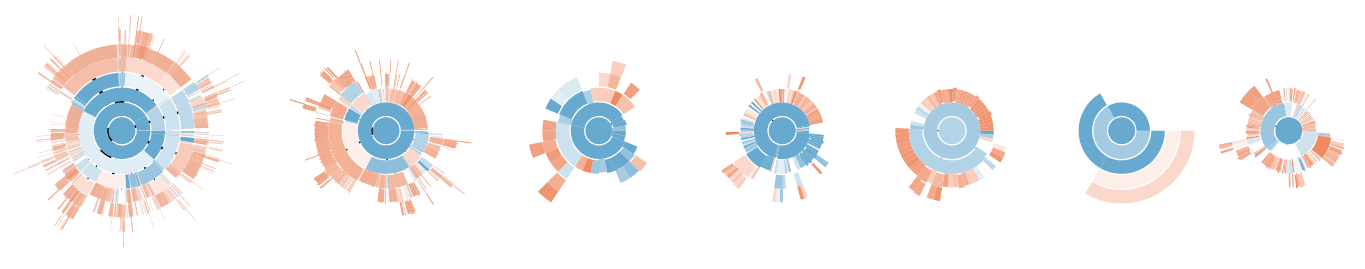
\includegraphics[width=\linewidth]{figs/current/burst_d2_top}
\caption{
Isolated neighborhoods shown as sunburst charts.
Each segment represents one data point.
The center indicates the data point with the highest score.
The distance to the center roughly corresponds with the number of changes
to the feature vector that are necessary to turn a point into the point at the center.
The size of the segments corresponds to the amount of points ``flowing"
through a point towards the center.
}
\label{figs:current_burst}
\end{figure}